\documentclass[conference]{IEEEtran}
\IEEEoverridecommandlockouts
% ------------------------------------------------------------------------------------------------
% CSI 5810 Midterm Project, Group 3 -- Bank Marketing (UCI dataset 222)
% Overleaf: upload this folder (main.tex, references.bib, figures/, tables/) and compile with pdfLaTeX.
% Every figure (figures/*.pdf) and table (tables/*.tex) is generated by code/bank_marketing_midterm.ipynb;
% the numbers quoted in the text come from code/outputs/results.json produced by the same run.
% ------------------------------------------------------------------------------------------------
\usepackage{cite}
\usepackage{amsmath,amssymb,amsfonts}
\usepackage{graphicx}
\usepackage{booktabs}
\usepackage{url}
\usepackage{xcolor}
\usepackage{textcomp}
\usepackage{eurosym}
\usepackage[T1]{fontenc}
\graphicspath{{figures/}}
\pdfminorversion=4
\pdfobjcompresslevel=0
% share (%) of test clients with calibrated GB probability above 0.7 (results.json: share_test_clients_p_above_0.7)
\newcommand{\pctHigh}{1.5}

\begin{document}

\title{Who Will Subscribe? Cost-Sensitive Prediction of Term-Deposit Subscription from Bank Telemarketing Data\\
{\large CSI 5810 Midterm Project, Group 3}}

\author{\IEEEauthorblockN{Andrew Aurand, Christina Carvalho, Cameron Clark, and Tyler Donovan}
\IEEEauthorblockA{Group 3, CSI 5810 Data Science and Big Data Analytics\\
Oakland University, Rochester, MI, USA\\
aaurand@oakland.edu}}

\maketitle

\begin{abstract}
We ask whether a Portuguese retail bank can predict, before a call is placed, which clients will subscribe to a term deposit, and whether targeting calls with such predictions lowers the expected campaign cost compared with calling everyone. Using the public UCI Bank Marketing data (41,188 clients, 11.3\% positives), we remove the post-outcome variable \texttt{duration} and compare a majority-class baseline with logistic regression, $k$-nearest neighbours, a random forest and histogram gradient boosting under a leakage-free, cross-validated protocol. Gradient boosting ranks best (test average precision 0.481, 95\% CI [0.445, 0.515]; ROC-AUC 0.810), but the tree ensembles are statistically indistinguishable and the linear model is only 0.03 AP behind. All models are well calibrated (expected calibration error $\le0.009$), so the Bayes-optimal rule ``call when the probability exceeds the cost ratio $c/v=0.10$'' applies directly: it calls 21\% of clients, reaches 65\% of subscribers and raises net value from \euro634 to \euro2,647 per 1,000 clients while cutting spend by 79\%. Sensitivity analyses show that the leakage variable would inflate ROC-AUC from 0.81 to 0.95, that class re-weighting destroys calibration without improving ranking, and that a model trained on earlier campaigns would have been worse than calling everyone on the later, higher-response campaigns unless re-calibrated, because the macro-economic inputs act as proxies for time.
\end{abstract}

\begin{IEEEkeywords}
bank marketing, imbalanced classification, cost-sensitive evaluation, probability calibration, precision--recall analysis, gradient boosting, concept drift
\end{IEEEkeywords}

\section{Introduction}
Direct-marketing calls consume agent time and telephony cost, yet only a small fraction of contacted clients buy the product: in the campaigns of the Portuguese bank studied here, roughly one client in nine subscribed to the term deposit on offer \cite{moro2014}. A model that ranks clients by their probability of subscribing could concentrate calls on the most likely subscribers, but only if the ranking is accurate, the probabilities are trustworthy enough to set a threshold, and the rule is judged by cost and return rather than by accuracy, which is meaningless when 89\% of clients say no.

\textbf{Research question.} \emph{Can we predict, before a call is placed, which clients will subscribe to a term deposit, and does using those predictions to target calls reduce the expected campaign cost compared with calling every client?}

\textbf{Contributions.} We (1)~document and audit the dataset, including a leakage variable; (2)~compare a majority-class baseline, logistic regression (LR), $k$-nearest neighbours ($k$-NN), a random forest (RF) and histogram gradient boosting (GB) under a leakage-free protocol; (3)~evaluate ranking, threshold metrics and calibration with bootstrap uncertainty; (4)~compare cost-based targeting policies with calling everyone; and (5)~analyse errors, subgroups and sensitivity to three modelling choices. A notebook reproducing every figure, table and number is submitted with this report.

\section{Dataset and Problem Definition}
\subsection{Source, provenance and permitted use}
We use the \emph{Bank Marketing} dataset of the UCI Machine Learning Repository (dataset~222), file \texttt{bank-additional-full.csv} \cite{uci_bank}, accessed on 30 September 2026. It is the (almost identical) public version of the data analysed in \cite{moro2014}: direct phone campaigns of a Portuguese bank between May~2008 and November~2010, ordered by date, with five national macro-economic indicators from Banco de Portugal merged by date. The data are released under the CC~BY~4.0 licence and contain no direct identifiers, only coarse client attributes and campaign metadata, so no additional privacy approval was needed. Known limitations: one bank and country, a period overlapping the 2008--2010 financial crisis, and a call volume that dropped sharply over time (Fig.~\ref{fig:target}).

\subsection{Unit of analysis, inputs, target and decision}
Each of the 41,188 rows is one client contacted in a campaign; the target $y$ is whether the client subscribed (\emph{yes} for 4,640 clients, 11.3\%). The 20 inputs (Table~\ref{tab:dictionary}, Appendix) fall into four families: seven client attributes (age, job, marital status, education, default, housing and personal loans), four attributes of the last contact (channel, month, weekday, duration), four campaign-history attributes (contacts in this campaign, days since and number of earlier contacts, previous outcome) and five macro-economic indicators (employment variation, consumer price and confidence indices, 3-month Euribor, number of employed). The task is binary classification with an uncommon positive class; the intended user is the campaign manager deciding \emph{which clients on the call list to contact}. We assume each contact costs $c$ and each subscription is worth $v$; the main scenario uses $c=$~\euro5 (agent time plus telephony) and $v=$~\euro50 (a \euro5,000 deposit at a 1\% net margin), a cost ratio $c/v=0.10$ that we vary from 0.05 to 0.30. Success means a ranking well above the base rate on the precision--recall curve, calibrated probabilities (expected calibration error below 0.02), and a targeting policy whose net value per 1,000 clients exceeds that of calling everyone, with bootstrap uncertainty.

\subsection{Data-quality audit and leakage}
The data have no missing cells, but several issues matter (full audit in Table~\ref{tab:audit}, Appendix). First, \texttt{duration} (seconds of the last call) is a \emph{leakage} variable \cite{kaufman2012}: it is only known after the call, and a zero-second call trivially implies ``no''. On its own it ranks subscribers with a ROC-AUC of 0.818; the dataset documentation says it must be discarded for a realistic model, and we do (Section~\ref{sec:sensitivity} quantifies the inflation). Second, 12 exact duplicate rows are removed. Third, missing values are coded as \texttt{unknown}: 20.9\% of rows for \texttt{default}, 4.2\% for \texttt{education}, 2.4\% for the loan flags and under 1\% for job and marital status. Because this missingness is informative (clients with unknown default status subscribe at 5.2\% versus 12.9\% for ``no''), \texttt{unknown} is kept as a category rather than imputed. Fourth, \texttt{pdays}=999 is a sentinel for ``never contacted before'' (96.3\% of rows). Fifth, a few clients were called up to 56 times and \texttt{default}=\emph{yes} occurs three times; neither is an error, so both are kept. Finally, the imbalance rules out accuracy as a criterion: predicting ``no'' for everyone is 88.7\% accurate and useless.

\section{Data Preparation and Exploratory Analysis}
\begin{figure*}[t]
\centering
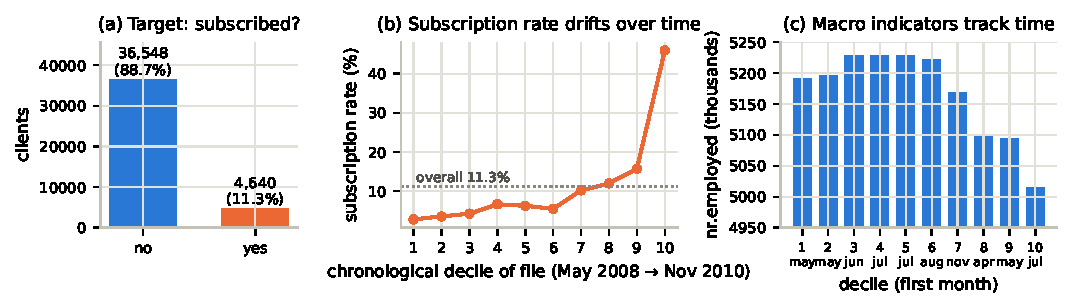
\includegraphics[width=0.78\textwidth]{fig_target_time.pdf}
\caption{(a) Class balance. (b) Subscription rate per chronological decile of the file (equal numbers of clients; the first six deciles cover May--November 2008, the last decile most of 2010). (c) The quarterly \texttt{nr.employed} indicator per decile: the macro-economic variables are step functions of time and act as proxies for the period in which a client was called.}
\label{fig:target}
\end{figure*}

\subsection{Exploratory analysis}
Fig.~\ref{fig:target} shows the two facts that shape the study. Only 11.3\% of clients subscribe, and the rate is far from stationary: it rises from 2.8\% in the earliest decile of the file (7,763 calls in May~2008 alone) to 45.9\% in the last decile (2010, when calls were few and better targeted). The macro-economic indicators are step functions of calendar time (Fig.~\ref{fig:target}(c)), so any model that uses them partly learns the calendar period rather than client behaviour.

Fig.~\ref{fig:cat} (Appendix) summarises the categorical variables. The previous campaign's outcome is the most informative attribute: 65.1\% of clients who accepted a previous offer subscribe again, versus 8.8\% of clients never contacted before. The channel matters (cellular 14.7\% vs.\ telephone 5.2\%), as does the month (above 43\% in the small March, September, October and December campaigns versus 6.4\% in May, the largest month). Students (31.4\%) and retired clients (25.2\%) subscribe most, blue-collar workers least (6.9\%). The numeric distributions by class (Fig.~\ref{fig:numeric}, Appendix) show subscribers over-represented below age 30 and above 60 and concentrated in the low-interest-rate regime. The correlation matrix (Fig.~\ref{fig:corr}, Appendix) shows that \texttt{euribor3m}, \texttt{nr.employed} and \texttt{emp.var.rate} are almost perfectly correlated ($r=0.91$--$0.97$) because they change only quarterly, and that they carry the strongest linear association with the target ($r=-0.30$ to $-0.35$). Cram\'er's $V$ ranks the categorical inputs \texttt{poutcome} (0.32) $>$ \texttt{month} (0.27) $>$ \texttt{job} (0.15) $>$ \texttt{contact} (0.14), all others below 0.1. Hence the macro-economic block should be read as one time-varying factor, and a chronological validation is needed to learn how a model behaves on a later campaign.

\subsection{Preparation and feature engineering}
Every preparation decision follows from the audit: \texttt{duration} and the 12 duplicates are dropped (41,176 clients remain); \texttt{pdays}=999 is replaced by~0 and a binary indicator \texttt{prev\_contacted} is added, so the linear model is not distorted by the sentinel while tree models keep the information; \texttt{unknown} is kept as a level; outliers are kept. Categorical variables are one-hot encoded; numeric variables are standardised for the linear and distance-based models, and gradient boosting receives ordinal codes with native categorical handling. All encoders and scalers live inside scikit-learn pipelines \cite{sklearn}, so they are fitted only on the training portion of each fold and never see validation or test data. We hold out a stratified 20\% test set (8,236 clients, 928 subscribers) that is used once, for the final numbers; all model selection (hyperparameters, decision thresholds and calibration maps) uses stratified 5-fold cross-validation inside the 80\% training set (32,940 clients). One seed (5810) controls every random step.

\section{Methods and Experimental Design}
\subsection{Baseline and comparison models}
\emph{Majority-class baseline}: predicts ``no'' for everyone and the class prior (0.113) as probability; the floor for every metric.
\emph{Logistic regression}: a linear model of the log-odds that assumes additive effects of the one-hot inputs and yields naturally calibrated probabilities; fast and interpretable. The L2 strength $C$ was tuned over $\{0.01,\dots,10\}$ (selected 3).
\emph{$k$-NN}: non-parametric and distance-based; assumes local smoothness in the standardised feature space and equally relevant features (doubtful with many weak one-hot features); cheap to fit, slow to predict. Tuned $k\in\{25,51,101,201\}$ and uniform vs.\ distance weights (selected $k=201$, uniform).
\emph{Random forest} \cite{breiman2001}: 300 bagged trees that capture interactions and are insensitive to scaling and outliers; probabilities are vote fractions. 18 random configurations of depth, leaf size and features per split were searched (selected depth~8, leaf~5, 50\% of features).
\emph{Histogram gradient boosting} \cite{friedman2001,ke2017}: additive trees fitted to log-loss gradients; strong on tabular data but prone to over-fitting. 24 random configurations of learning rate, leaves, leaf size, L2 penalty and rounds were searched (selected rate 0.03, 15 leaves, leaf 100, 150 rounds: a strongly regularised, shallow model). Grids are listed in Table~\ref{tab:grids} (Appendix). The expected trade-off is interpretability and speed (LR) against capacity (RF, GB), with $k$-NN as a cheap reference.

\subsection{Evaluation protocol}
Average precision (AP, area under the precision--recall curve) is the selection score because it focuses on the rare positive class and needs no threshold \cite{saito2015}; ROC-AUC and the Brier score are recorded alongside, with fold-to-fold standard deviations. On the test set we report AP, ROC-AUC (the probability that a random subscriber outranks a random non-subscriber), the Brier score (mean squared error of the probabilities \cite{brier1950}), log loss and expected calibration error (ECE, the average gap between predicted and observed subscription frequency over ten equal-width bins \cite{naeini2015}), each with a 95\% bootstrap confidence interval from 1,000 resamples of the test rows \cite{efron1993}; the same resamples serve every model, so differences are paired. Threshold metrics and confusion matrices are reported at the library default $t=0.5$, at a threshold tuned on out-of-fold training predictions, and at the cost-based threshold below.

\subsection{Calibration and cost model}
A cost-based rule is only valid if the probabilities are calibrated: among clients given $p=0.2$, about 20\% should subscribe \cite{niculescu2005}. We assess calibration with reliability diagrams, Brier score and ECE, and fit isotonic-regression calibrators \cite{zadrozny2002} by 5-fold cross-validation inside the training set, so the test set stays untouched. Calling client $i$ costs $c$ and a subscription earns $v$. A policy that calls the clients with $p_i\ge t$, producing TP true and FP false positives and FN false negatives, spends $c\,(\mathrm{TP}+\mathrm{FP})$ and earns a \emph{net value} $v\,\mathrm{TP}-c\,(\mathrm{TP}+\mathrm{FP})$. Its misclassification cost relative to perfect targeting is $c\,\mathrm{FP}+(v-c)\,\mathrm{FN}$; minimising it is equivalent to maximising net value. For calibrated probabilities the Bayes-optimal rule is to call whenever $p_i v\ge c$, i.e.\ $t^\star=c/v=0.10$ \cite{elkan2001}. Amounts are reported per 1,000 clients and compared with calling nobody, calling everyone (current practice) and a perfect-information oracle.

\section{Results and Discussion}
\subsection{Model comparison}
\begin{table}[t]
\caption{Model comparison: 5-fold cross-validated AP on the training set (mean $\pm$ s.d.) and test-set metrics (8,236 clients, 928 subscribers) with 95\% bootstrap confidence intervals.}
\label{tab:models}
\centering\scriptsize
\setlength{\tabcolsep}{3pt}
\resizebox{\columnwidth}{!}{\begin{tabular}{lcccc}
\toprule
model & CV AP (mean $\pm$ sd) & test AP [95\% CI] & test ROC-AUC [95\% CI] & test Brier [95\% CI] \\
\midrule
Majority baseline & 0.113 $\pm$ 0.000 & 0.113 [0.113, 0.113] & 0.500 [0.500, 0.500] & 0.100 [0.100, 0.100] \\
Logistic regression & 0.453 $\pm$ 0.012 & 0.449 [0.416, 0.486] & 0.796 [0.778, 0.814] & 0.079 [0.074, 0.083] \\
k-NN & 0.433 $\pm$ 0.016 & 0.434 [0.400, 0.471] & 0.791 [0.773, 0.807] & 0.079 [0.075, 0.084] \\
Random forest & 0.469 $\pm$ 0.016 & 0.479 [0.444, 0.514] & 0.806 [0.789, 0.823] & 0.077 [0.072, 0.081] \\
Gradient boosting & 0.472 $\pm$ 0.016 & 0.481 [0.445, 0.515] & 0.810 [0.794, 0.827] & 0.076 [0.072, 0.081] \\
\bottomrule
\end{tabular}}
\end{table}

\begin{figure*}[t]
\centering
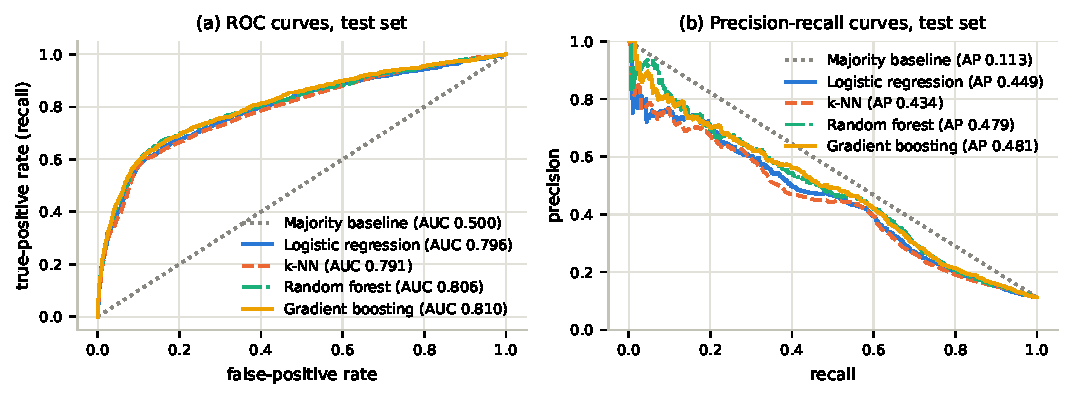
\includegraphics[width=0.68\textwidth]{fig_roc_pr.pdf}
\caption{(a) ROC and (b) precision--recall curves on the test set. The baseline's PR ``curve'' is the base rate; the learned models are close, with the tree ensembles slightly ahead at low recall.}
\label{fig:rocpr}
\end{figure*}

Table~\ref{tab:models} and Fig.~\ref{fig:rocpr} summarise ranking quality. Gradient boosting is selected by cross-validated AP ($0.472\pm0.016$) but is tied with the random forest ($0.469\pm0.016$); both beat LR ($0.453$) by about 0.02 and $k$-NN ($0.433$) by about 0.04, differences comparable to the fold-to-fold standard deviation. On the untouched test set GB reaches AP 0.481 [0.445, 0.515], 4.3 times the base rate, and ROC-AUC 0.810 [0.794, 0.827]. The paired bootstrap confirms the picture: GB minus LR is $+0.031$ AP [+0.018, +0.045], GB minus $k$-NN $+0.046$ [+0.032, +0.061], but GB minus RF only $+0.001$ [$-0.008$, $+0.010$]. The precision--recall curve shows the limits of the ranking: precision is 0.6--0.7 at recall 0.2--0.3, about 0.35 when two thirds of subscribers are reached, and it decays to the base rate at full recall. The information available before a call supports a useful but imperfect ranking; much of the outcome depends on the call itself, which is what the excluded \texttt{duration} variable encodes.

\subsection{Calibration}
\begin{figure*}[t]
\centering
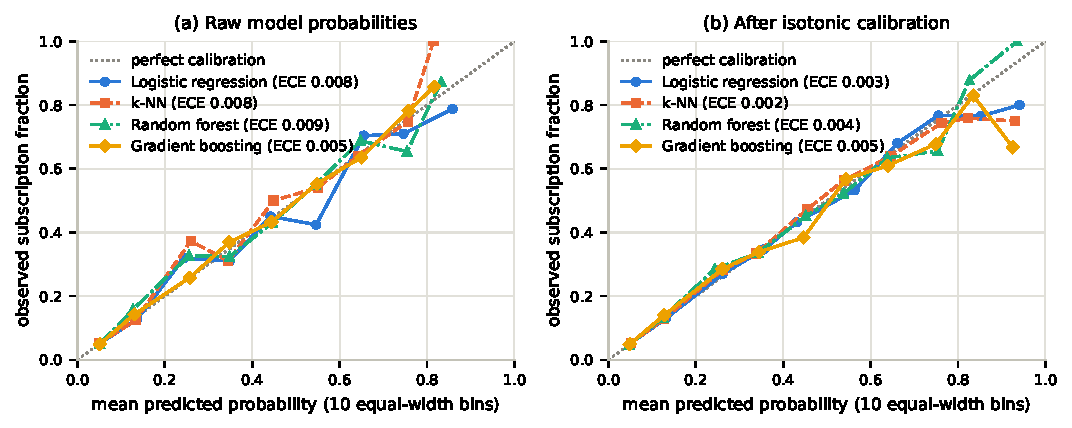
\includegraphics[width=0.68\textwidth]{fig_calibration.pdf}
\caption{Reliability diagrams on the test set (a) for the raw model probabilities and (b) after isotonic calibration fitted by cross-validation inside the training set. ECE = expected calibration error (10 equal-width bins).}
\label{fig:cal}
\end{figure*}

Fig.~\ref{fig:cal} shows that all four models are already well calibrated without post-processing: ECE is 0.005 (GB) to 0.009 (RF), the mean predicted probability equals the prevalence (0.112), and Brier scores (0.076--0.079) are well below the 0.100 of predicting the prior. No model used re-weighting or resampling, which would have distorted the probabilities (Section~\ref{sec:sensitivity} shows the effect). Isotonic calibration lowers ECE to 0.002--0.005 and changes Brier scores by at most 0.0003 and AP by at most 0.004; the wiggles above $p=0.7$ are sampling noise, since only about \pctHigh\% of test clients receive such probabilities. The decision rule below uses the calibrated models.

\subsection{Cost-sensitive evaluation}
\begin{figure*}[t]
\centering
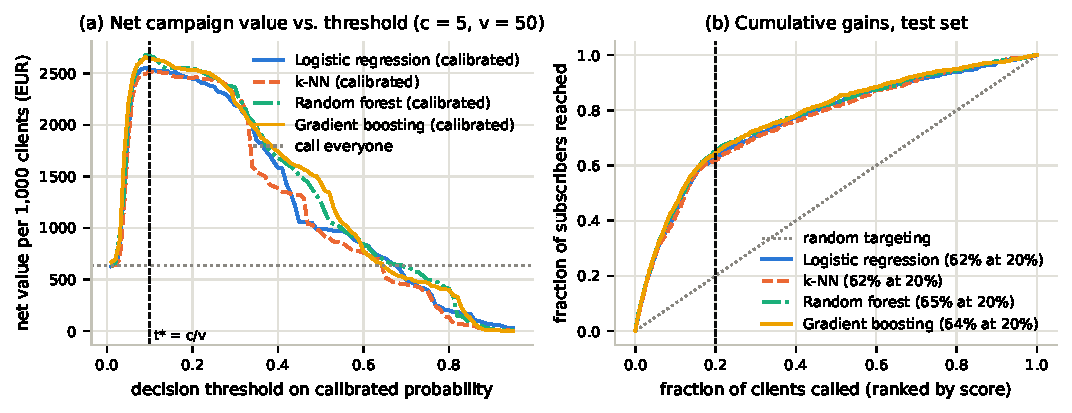
\includegraphics[width=0.68\textwidth]{fig_cost_gains.pdf}
\caption{(a) Net campaign value per 1,000 clients versus the decision threshold applied to calibrated probabilities ($c=$~\euro5, $v=$~\euro50); the dotted line is calling everyone, the dashed line the Bayes threshold $t^\star=c/v$. (b) Cumulative gains: share of all subscribers reached when the top fraction of clients by score is called.}
\label{fig:cost}
\end{figure*}

\begin{table}[t]
\caption{Campaign policies on the test set, per 1,000 clients ($c=$~\euro5 per call, $v=$~\euro50 per subscription). Model rows use calibrated probabilities with the Bayes threshold $t^\star=0.10$.}
\label{tab:strat}
\centering\scriptsize
\setlength{\tabcolsep}{3pt}
\resizebox{\columnwidth}{!}{\begin{tabular}{lrrrrr}
\toprule
strategy & call rate & precision & recall & spend / 1,000 & net value / 1,000 \\
\midrule
Call nobody & 0.00 & 0.00 & 0.00 & 0 & 0 \\
Call everyone & 1.00 & 0.11 & 1.00 & 5,000 & 634 \\
Oracle (perfect information) & 0.11 & 1.00 & 1.00 & 563 & 5,070 \\
Logistic regression (calibrated) & 0.21 & 0.35 & 0.63 & 1,030 & 2,534 \\
k-NN (calibrated) & 0.20 & 0.36 & 0.62 & 979 & 2,518 \\
Random forest (calibrated) & 0.22 & 0.34 & 0.67 & 1,096 & 2,668 \\
Gradient boosting (calibrated) & 0.21 & 0.35 & 0.65 & 1,038 & 2,647 \\
\bottomrule
\end{tabular}}
\end{table}

\begin{table}[t]
\caption{Net value per 1,000 clients for different cost ratios $c/v$ (calibrated models, threshold $t^\star=c/v$) and the share of clients called by the GB rule.}
\label{tab:ratio}
\centering\scriptsize
\setlength{\tabcolsep}{3pt}
\resizebox{\columnwidth}{!}{\begin{tabular}{lrrrrrr}
\toprule
c/v & call everyone & LR & k-NN & RF & GB & call rate (GB) \\
\midrule
0.05 & 3,134 & 3,446 & 3,381 & 3,416 & 3,471 & 0.51 \\
0.10 & 634 & 2,534 & 2,518 & 2,668 & 2,647 & 0.21 \\
0.20 & -4,366 & 1,702 & 1,695 & 1,809 & 1,786 & 0.15 \\
0.30 & -9,366 & 1,003 & 948 & 1,084 & 1,068 & 0.11 \\
\bottomrule
\end{tabular}}
\end{table}

In Fig.~\ref{fig:cost}(a) every curve peaks between $t=0.08$ and $0.12$, where the thresholds tuned on out-of-fold training predictions also fall (0.09 for RF and GB, 0.11 for $k$-NN, 0.13 for LR): calibrated probabilities plus the Bayes rule recover the empirically optimal operating point without tuning. Table~\ref{tab:strat} compares policies. Calling everyone spends \euro5,000 per 1,000 clients for a net value of only \euro634; its misclassification cost is \euro4,437. The calibrated GB rule calls 20.8\% of clients, reaches 65.4\% of subscribers at 35.5\% precision, spends \euro1,038 and nets \euro2,647 per 1,000 clients, 4.2 times the value of calling everyone with one fifth of the budget, and cuts the misclassification cost by 45\% to \euro2,424. All four learned models land within \euro150 of each other (RF \euro2,668, LR \euro2,534, $k$-NN \euro2,518): using any calibrated model with a cost-based threshold matters far more than the choice among models. The gains curve (Fig.~\ref{fig:cost}(b)) gives the budget-constrained view: the top 20\% of clients by GB score contain 64\% of all subscribers and the top 40\% contain 78\%. Table~\ref{tab:ratio} varies the cost ratio: model targeting dominates everywhere, calling everyone loses money once $c/v$ exceeds the base rate (0.113), and the GB rule stays profitable throughout by shrinking its call list from 51\% of clients at $c/v=0.05$ to 11\% at $c/v=0.30$.

\subsection{Operating points and confusion matrices}
\begin{table}[t]
\caption{Confusion matrices of gradient boosting on the test set at the default threshold and for the recommended calibrated rule.}
\label{tab:cm}
\centering\scriptsize
\begin{tabular}{lrrcrr}
\toprule
 & \multicolumn{2}{c}{raw, $t=0.5$} & & \multicolumn{2}{c}{calibrated, $t^\star=0.10$} \\
\cmidrule{2-3}\cmidrule{5-6}
 & pred.\ no & pred.\ yes & & pred.\ no & pred.\ yes \\
\midrule
true no & 7,186 & 122 & & 6,205 & 1,103 \\
true yes & 689 & 239 & & 321 & 607 \\
\bottomrule
\end{tabular}
\end{table}

Table~\ref{tab:cm} shows how much the threshold matters. At the library default of 0.5, GB has an accuracy of 0.901, barely above the 0.887 of always predicting ``no'', because it calls only 4.4\% of clients; precision is high (0.662) but recall is 0.258 (689 false negatives), balanced accuracy 0.620, F1 0.371, and the net value \euro1,232 per 1,000. The cost-based rule accepts lower accuracy (0.827) and precision (0.355) for recall 0.654, specificity 0.849, balanced accuracy 0.752, F1 0.460 and more than twice the net value. The confusion matrix makes the asymmetry of errors explicit: a false positive wastes one \euro5 call, a false negative forgoes \euro45 of margin, so the optimal rule deliberately tolerates about two wasted calls per subscriber found.

\section{Error Analysis, Limitations, and Responsible Use}
\subsection{What drives the predictions}
Fig.~\ref{fig:imp}(a) (Appendix) ranks the inputs by permutation importance \cite{breiman2001}, the drop in test AP when one column is shuffled. The quarterly employment indicator \texttt{nr.employed} dominates (drop 0.167), followed by \texttt{month} (0.052), \texttt{emp.var.rate} (0.025), the contact channel (0.023), whether and how the client was contacted before (0.018 and 0.017), then weekday, Euribor, number of calls and age (0.015--0.005); job, education, marital status and the loan flags contribute less than 0.002 each. The model therefore mostly learns when the client was called (macro regime and month) and how (channel, previous outcome, number of attempts), not who the client is. The logistic coefficients (Fig.~\ref{fig:imp}(b)) add signs: one standard deviation of employment variation multiplies the odds of subscribing by $e^{-2.19}\approx0.11$, the March indicator multiplies them by 3.5, and telephone contact, a failed previous campaign, undisclosed default status and Monday calls all lower them. \texttt{nr.employed} and \texttt{euribor3m} receive positive coefficients despite negative marginal correlations: with $r>0.9$ among the macro indicators only their joint effect is interpretable. Partial-dependence curves \cite{friedman2001} (Fig.~\ref{fig:pdp}, Appendix) show the probability falling from 0.12 at one or two calls to 0.03 beyond about 18 calls, and a mild U-shape in age.

\subsection{Concrete errors and error patterns}
\begin{table}[t]
\caption{Most confident correct decisions (TP: called and subscribed; TN: not called, did not subscribe) and mistakes (FN: subscribed, not called; FP: called, did not subscribe) of the calibrated GB rule on the test set; ``prob.'' is the calibrated probability.}
\label{tab:examples}
\centering\scriptsize
\setlength{\tabcolsep}{3pt}
\resizebox{\columnwidth}{!}{\begin{tabular}{llllllrrr}
\toprule
type & age & job & contact & month & poutcome & calls & euribor3m & prob. \\
\midrule
TP & 92 & retired & cellular & aug & success & 1 & 0.90 & 0.923 \\
TP & 37 & unemployed & cellular & jul & success & 1 & 0.88 & 0.914 \\
TN & 52 & management & telephone & may & nonexistent & 35 & 4.86 & 0.000 \\
TN & 38 & blue-collar & telephone & jun & nonexistent & 41 & 4.96 & 0.000 \\
FN & 39 & blue-collar & telephone & may & nonexistent & 23 & 4.86 & 0.000 \\
FN & 44 & blue-collar & telephone & may & nonexistent & 1 & 4.86 & 0.017 \\
FP & 39 & admin. & cellular & mar & success & 1 & 0.65 & 0.939 \\
FP & 33 & self-employed & cellular & mar & success & 1 & 0.64 & 0.862 \\
\bottomrule
\end{tabular}}
\end{table}

Table~\ref{tab:examples} lists the most confident decisions of each kind. The confident correct decisions are easy cases: true positives are previous-campaign successes reached by mobile in 2010 ($p=0.92$ and $0.91$); true negatives are clients called 35 and 41 times by landline in mid-2008 without success ($p=0.00$). The worst false negatives are blue-collar clients with basic education, contacted by landline in May~2008 (Euribor 4.86\%) with no earlier campaign; every attribute places them in the lowest-rate groups, so the calibrated model estimates $p\le0.02$, and nothing in the inputs distinguishes the few who subscribe. The most confident false positives ($p=0.86$--$0.94$) are clients whose previous campaign succeeded, reached by mobile phone in the low-rate 2010 period, a group with a 64\% subscription rate, so one miss in three is expected and costs one call. Errors also cluster in time: recall of the rule is lowest in the high-volume months May (45\%, prevalence 6.7\%) and July (35\%), whereas in March, September and October the month alone pushes $p$ above 0.10, so the rule calls every client (prevalence 44--52\%).

\subsection{Subgroup performance and fairness}
Fig.~\ref{fig:sub} and Table~\ref{tab:subgroups} (Appendix) break the rule down by subgroup. Precision is fairly uniform (0.30--0.36) across groups with ordinary base rates, but recall is not: the rule reaches 99\% of subscribers aged 60+ (prevalence 46\%) and 73\% of those under 30, but only 57--58\% of clients aged 30--59; 70\% of subscribers reached by mobile but 42\% of those reached by landline; 70\% of clients with a known default status but 16\% of those with an undisclosed one; 92\% of students and 89\% of retired clients against 38\% of blue-collar and 32\% of service workers. The pattern follows directly from the Bayes rule: groups with low base rates are called less, so their subscribers are missed more often. It is optimal in expected value, but it concentrates the bank's offers on older, previously engaged, mobile-reachable clients and under-serves groups such as blue-collar workers. Age and employment are sensitive attributes, so this allocation should be an explicit business and ethics decision, e.g.\ monitored through recall per group or adjusted with group-specific thresholds.

\subsection{Sensitivity to modelling choices}\label{sec:sensitivity}
\begin{table}[t]
\caption{Effect of three modelling choices on the test set (random split unless stated). Rows with \texttt{duration} are unrealistic (leakage); the temporal split trains on the first 80\% of clients in time and tests on the last 20\%.}
\label{tab:sens}
\centering\scriptsize
\setlength{\tabcolsep}{3pt}
\resizebox{\columnwidth}{!}{\begin{tabular}{lrrrrr}
\toprule
experiment & model & AP & ROC-AUC & Brier & ECE \\
\midrule
leakage: with duration & Logistic regression & 0.595 & 0.935 & 0.064 & 0.031 \\
main: without duration & Logistic regression & 0.449 & 0.796 & 0.079 & 0.008 \\
leakage: with duration & Gradient boosting & 0.667 & 0.950 & 0.056 & 0.008 \\
main: without duration & Gradient boosting & 0.481 & 0.810 & 0.076 & 0.005 \\
temporal split (last 20\% as test) & Logistic regression & 0.526 & 0.748 & 0.191 & 0.097 \\
temporal split (last 20\% as test) & Gradient boosting & 0.482 & 0.676 & 0.232 & 0.190 \\
temporal split, calibrated & Gradient boosting & 0.482 & 0.665 & 0.234 & 0.190 \\
class\_weight = balanced & Logistic regression & 0.444 & 0.797 & 0.162 & 0.275 \\
class\_weight = balanced & Gradient boosting & 0.476 & 0.811 & 0.155 & 0.266 \\
\bottomrule
\end{tabular}}
\end{table}

\emph{Leakage.} Adding \texttt{duration} raises ROC-AUC from 0.810 to 0.950 and AP from 0.481 to 0.667 for GB (0.796 to 0.934 and 0.449 to 0.595 for LR; Table~\ref{tab:sens}). Those numbers would mean nothing in deployment, because the variable does not exist when the decision is made.

\emph{Temporal validation.} Training on the chronologically first 80\% of clients and testing on the last 20\% simulates deployment on a future campaign. The training prevalence is 6.4\%, the test prevalence 30.8\%, and 60\% of test rows carry \texttt{nr.employed} values (98.5\% Euribor values) never seen in training. The ranking survives (GB AP 0.482, LR 0.526, both above the new base rate), but the probabilities do not: ROC-AUC falls to 0.676 (GB) and 0.748 (LR), the Brier score of GB (0.232) is worse than predicting the prior, and ECE stays at 0.19 even after calibration, because the isotonic map was itself learned in the old regime. In money terms (Table~\ref{tab:temporal}, Appendix), calling everyone in the later campaigns nets \euro10,414 per 1,000 clients, whereas the GB rule at $t^\star$ nets only \euro6,059 (calibrated) or \euro6,263 (raw), because it under-predicts probabilities and calls too few clients (28\%, recall 48\%). A model trained on 2008--2009 and applied unchanged in 2010 would have been worse than no model; the tree ensemble degrades more than the linear model because it cannot extrapolate beyond the macro-indicator values it has seen. The random-split results are therefore an upper bound on deployable performance, and deployment needs re-calibration on fresh outcomes and drift monitoring \cite{morenotorres2012}.

\emph{Class weighting.} Re-fitting LR and GB with \texttt{class\_weight=balanced} leaves the ranking unchanged (AP 0.444 vs.\ 0.449 and 0.476 vs.\ 0.481) but destroys calibration: Brier rises to 0.16 and ECE to 0.27, and with the Bayes threshold the weighted models call 99\% of clients (net \euro639--667, as for calling everyone). At $t=0.5$ they call 19--20\% of clients and net \euro2,521--2,614: weighting merely moves the operating point that an explicit threshold already controls, while making the probabilities unusable.

\subsection{Limitations, responsible use and next steps}
The data come from one bank, one country and one unusual period, and the public file omits some attributes of the original study, so results will not transfer without re-training. The macro-economic inputs are time proxies, so random-split estimates are optimistic. The cost parameters are illustrative; the bank should insert its own (Table~\ref{tab:ratio}). \texttt{campaign} counts calls including the last one, so the model is best read as deciding whether to (re)contact a client at each attempt. Hyperparameters tuned on the random split were reused for the temporal check; all intervals come from a single test split; and without client identifiers repeated clients cannot be tracked. Computation is not a constraint (the whole pipeline runs in about five minutes on a laptop) and one fixed seed makes every number reproducible. The model should serve as decision support for prioritising calls, not for denying service, with probabilities re-calibrated at the start of every campaign and recall audited by subgroup; only the public, de-identified attributes were used. Next steps: (1)~rolling, time-ordered validation with the calibration map re-fitted on the first weeks of each campaign; (2)~testing transferability without the macro block; (3)~uplift modelling, since clients with a successful previous campaign may subscribe anyway; (4)~a budget-constrained formulation with per-attempt costs.

\section{Conclusion}
Before a call is placed, the available information supports a useful but modest ranking of clients: gradient boosting reaches a test average precision of 0.48 (4.3 times the base rate) and a ROC-AUC of 0.81, with the other learners close behind. What turns this ranking into value is the decision rule rather than the learner: because all models are well calibrated, the Bayes threshold $t^\star=c/v=0.10$ calls one fifth of the clients, reaches two thirds of the subscribers and raises net value from \euro634 to \euro2,647 per 1,000 clients while cutting spend by 79\%. The main risk is drift: the strongest predictors are macro-economic proxies for time, and a model trained on earlier campaigns would have lost money relative to calling everyone on the later ones unless re-calibrated. The answer to our question is a qualified yes: targeting with calibrated probabilities and an explicit cost threshold substantially reduces expected campaign cost on contemporaneous data, provided the model is monitored and re-calibrated as conditions change.

\section*{Contribution Statement}
\textcolor{red}{[Confirm the role split with the group and remove this note before submission.]}
\textbf{Andrew Aurand} (coordinator, graduate student): research question and cost-model design, shared workspace and project log, notebook integration, final editing. \textbf{Christina Carvalho} (data-preparation lead): data documentation, quality audit, preparation pipelines and leakage controls, exploratory figures. \textbf{Cameron Clark} (modeling lead): model implementations, hyperparameter search, calibration, feature-importance and partial-dependence analysis. \textbf{Tyler Donovan} (evaluation lead): test-set evaluation, bootstrap intervals, cost-sensitive evaluation, error, subgroup and sensitivity analyses. All members wrote and reviewed the report sections corresponding to their work.

\section*{Generative-AI Disclosure}
Anthropic's Claude (Claude Code) was used to draft and debug the analysis notebook, to structure the experiments, and to draft and edit the report text and LaTeX. All generated code, results, explanations and citations were reviewed by the group, which is responsible for all methodological choices, the interpretation and the conclusions. A meeting record and task-ownership log is submitted with the code archive.

\bibliographystyle{IEEEtran}
\bibliography{references}

\clearpage
\appendix
This appendix collects the supporting material referenced in the text: the categorical exploratory figure, the data-quality audit, the hyperparameter grids, the cost view of the temporal split, the correlation matrix, the numeric distributions by class, the data dictionary, the feature-importance and partial-dependence figures, and the full subgroup table.

\begin{figure*}[!t]
\centering
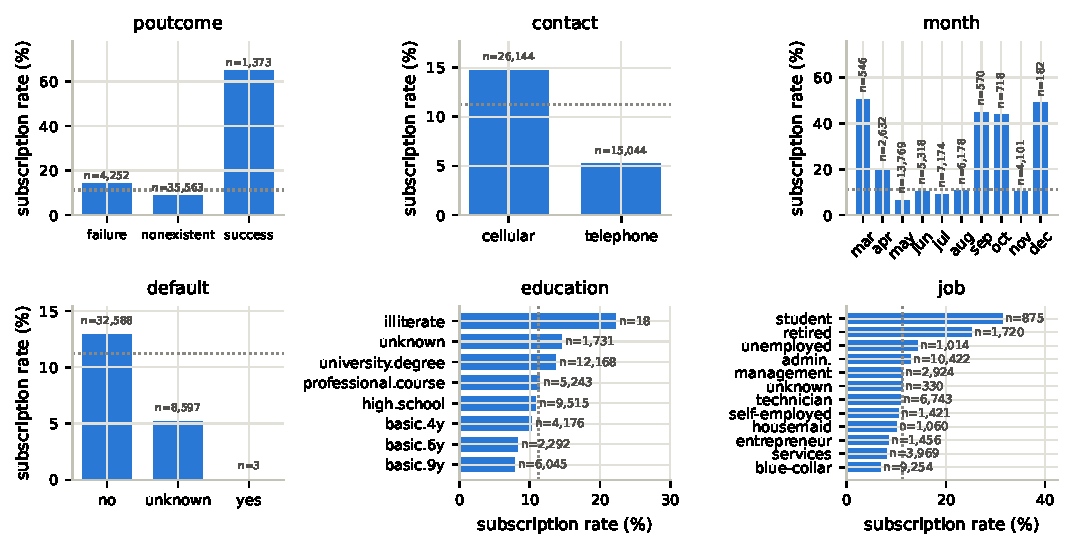
\includegraphics[width=\textwidth]{fig_categorical_rates.pdf}
\caption{Subscription rate (\%) by categorical variable with group sizes $n$; the dotted line is the overall rate of 11.3\%. Previous-campaign success, the cellular channel and the low-volume months are the strongest categorical signals; students and retired clients subscribe far more often than blue-collar workers.}
\label{fig:cat}
\end{figure*}

\begin{table}[!h]
\caption{Data-quality audit of \texttt{bank-additional-full.csv} (41,188 rows; notebook Section~3).}
\label{tab:audit}
\centering\scriptsize
\resizebox{\columnwidth}{!}{\begin{tabular}{p{0.42\linewidth}p{0.52\linewidth}}
\toprule
check & finding \\
\midrule
Rows / columns & 41,188 / 21 \\
Exact duplicate rows & 12 (dropped) \\
Positive class (y = yes) & 4,640 (11.3\%) \\
Rows with any 'unknown' value & 10,700 (26.0\%) \\
'unknown' by column & default 8,597, education 1,731, housing 990, loan 990, job 330, marital 80 \\
pdays = 999 (never contacted before) & 96.3\% of rows \\
duration = 0 s & 4 rows, all y = no \\
ROC-AUC of duration alone & 0.818 (leakage; feature dropped) \\
campaign > 10 contacts & 869 rows (max 56) \\
age > 80 & 119 rows \\
default = yes & 3 rows (level kept, effectively 'no' vs 'unknown') \\
\bottomrule
\end{tabular}}
\end{table}

\begin{table}[!h]
\caption{Hyperparameter search spaces and selected values (5-fold CV, average precision).}
\label{tab:grids}
\centering\scriptsize
\setlength{\tabcolsep}{3pt}
\resizebox{\columnwidth}{!}{\begin{tabular}{llll}
\toprule
model & hyperparameter & candidates & selected \\
\midrule
Logistic regression & C & [0.01, 0.03, 0.1, 0.3, 1.0, 3.0, 10.0] & 3.0 \\
k-NN & n\_neighbors & [25, 51, 101, 201] & 201 \\
k-NN & weights & ['uniform', 'distance'] & uniform \\
Random forest & max\_depth & [8, 12, 16, None] & 8 \\
Random forest & min\_samples\_leaf & [1, 5, 20] & 5 \\
Random forest & max\_features & ['sqrt', 0.3, 0.5] & 0.5 \\
Gradient boosting & learning\_rate & [0.03, 0.06, 0.1] & 0.03 \\
Gradient boosting & max\_leaf\_nodes & [15, 31, 63] & 15 \\
Gradient boosting & min\_samples\_leaf & [20, 50, 100] & 100 \\
Gradient boosting & l2\_regularization & [0.0, 1.0, 5.0] & 0.0 \\
Gradient boosting & max\_iter & [150, 300, 500] & 150 \\
\bottomrule
\end{tabular}}
\end{table}

\begin{table}[!h]
\caption{Cost view of the temporal split (last 20\% of the file as test set, prevalence 30.8\%), per 1,000 clients.}
\label{tab:temporal}
\centering\scriptsize
\setlength{\tabcolsep}{3pt}
\begin{tabular}{lrrrr}
\toprule
policy (temporal test set) & call rate & precision & recall & net value / 1,000 \\
\midrule
call everyone & 1.00 & 0.31 & 1.00 & 10,414 \\
GB, raw, t* = 0.10 & 0.29 & 0.53 & 0.50 & 6,263 \\
GB, calibrated, t* = 0.10 & 0.28 & 0.54 & 0.48 & 6,059 \\
\bottomrule
\end{tabular}
\end{table}

\begin{figure}[!t]
\centering
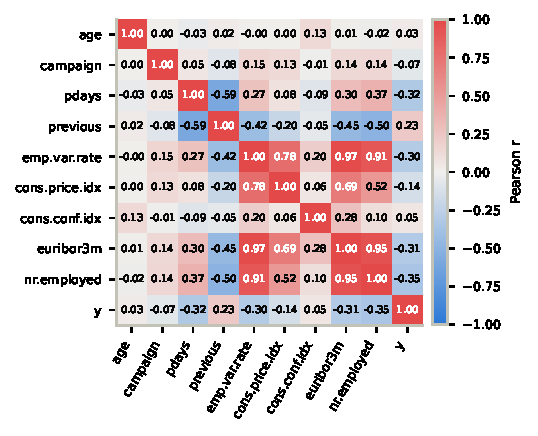
\includegraphics[width=\columnwidth]{fig_correlation.pdf}
\caption{Pearson correlation among the numeric inputs and the binary target. The three quarterly macro indicators are almost collinear ($r\ge0.91$) and carry the largest linear association with the target.}
\label{fig:corr}
\end{figure}

\begin{figure}[!t]
\centering
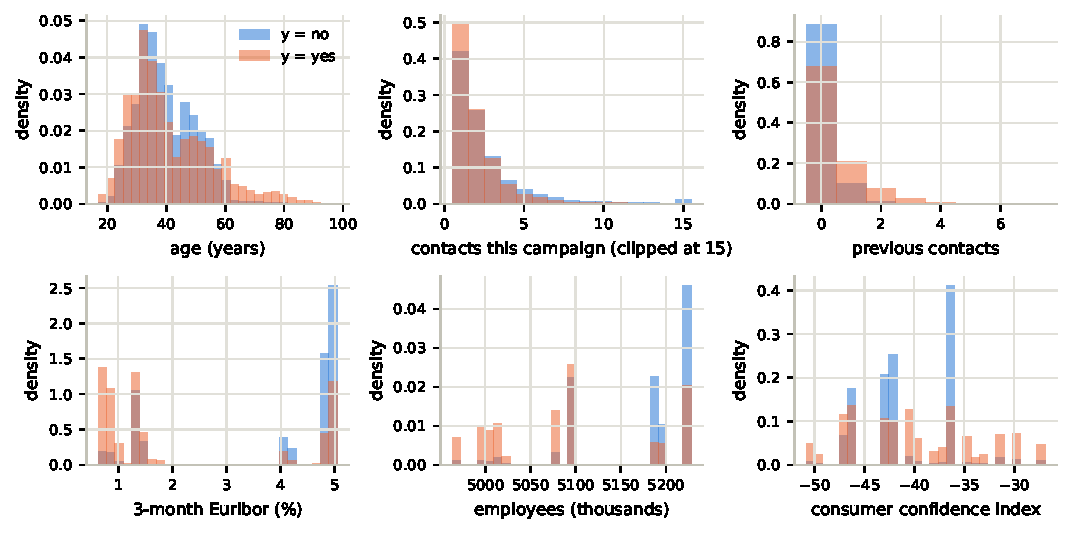
\includegraphics[width=\columnwidth]{fig_numeric_by_class.pdf}
\caption{Distributions of important numeric variables by class (densities; \texttt{campaign} clipped at 15 for display).}
\label{fig:numeric}
\end{figure}

\begin{table*}[!t]
\caption{Data dictionary of the Bank Marketing dataset (\texttt{bank-additional-full.csv}); ``unknown'' is the number of rows with the missing-value label.}
\label{tab:dictionary}
\centering\scriptsize
\begin{tabular}{llllrl}
\toprule
variable & group & type & levels / range & unknown & description \\
\midrule
age & client & numeric & 17 - 98 & 0 & client age in years \\
job & client & categorical & 12 levels & 330 & type of job (12 levels) \\
marital & client & categorical & 4 levels & 80 & marital status \\
education & client & categorical & 8 levels & 1731 & highest education level (8 levels) \\
default & client & categorical & 3 levels & 8597 & has credit in default? \\
housing & client & categorical & 3 levels & 990 & has a housing loan? \\
loan & client & categorical & 3 levels & 990 & has a personal loan? \\
contact & last contact & categorical & 2 levels & 0 & contact communication type (cellular / telephone) \\
month & last contact & categorical & 10 levels & 0 & month of last contact \\
day\_of\_week & last contact & categorical & 5 levels & 0 & weekday of last contact \\
duration & last contact & numeric & 0 - 4918 & 0 & last-call duration in seconds (LEAKAGE: known only after the call; dropped) \\
campaign & campaign history & numeric & 1 - 56 & 0 & number of contacts in this campaign for this client (incl. last) \\
pdays & campaign history & numeric & 0 - 999 & 0 & days since last contact in a previous campaign (999 = never contacted) \\
previous & campaign history & numeric & 0 - 7 & 0 & number of contacts before this campaign \\
poutcome & campaign history & categorical & 3 levels & 0 & outcome of the previous campaign (failure / nonexistent / success) \\
emp.var.rate & macro-economic & numeric & -3.4 - 1.4 & 0 & employment variation rate, quarterly (\%) \\
cons.price.idx & macro-economic & numeric & 92.201 - 94.767 & 0 & consumer price index, monthly \\
cons.conf.idx & macro-economic & numeric & -50.8 - -26.9 & 0 & consumer confidence index, monthly \\
euribor3m & macro-economic & numeric & 0.634 - 5.045 & 0 & 3-month Euribor rate, daily (\%) \\
nr.employed & macro-economic & numeric & 4963.6 - 5228.1 & 0 & number of employees, quarterly (thousands) \\
y & target & categorical & 2 levels & 0 & TARGET: subscribed a term deposit? (yes / no) \\
\bottomrule
\end{tabular}
\end{table*}

\begin{figure*}[!t]
\centering
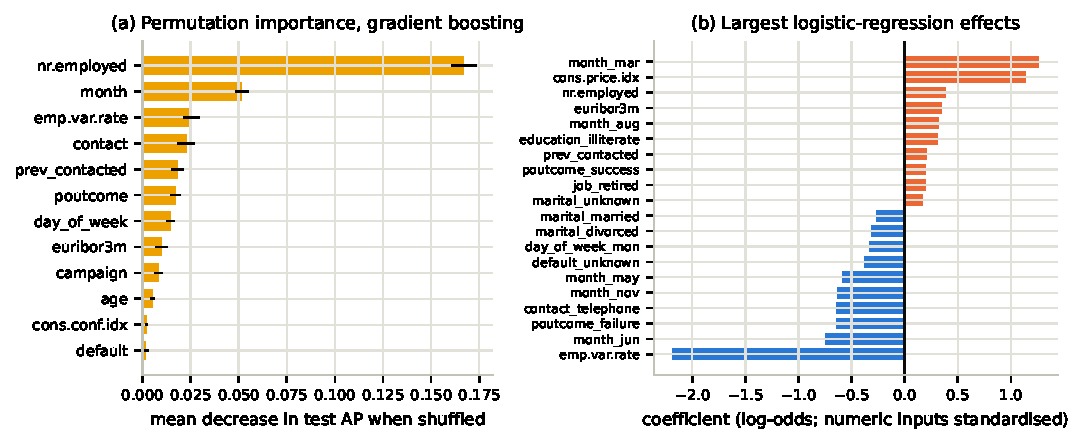
\includegraphics[width=0.9\textwidth]{fig_importance.pdf}
\caption{(a) Permutation importance of the selected gradient-boosting model (mean decrease in test AP over 10 shuffles, with s.d.). (b) The ten most negative and ten most positive logistic-regression coefficients.}
\label{fig:imp}
\end{figure*}

\begin{figure*}[!t]
\centering
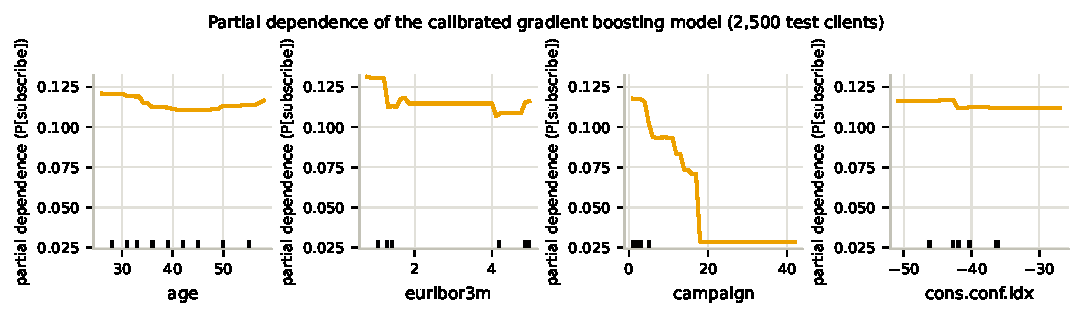
\includegraphics[width=0.95\textwidth]{fig_pdp.pdf}
\caption{Partial dependence of the calibrated gradient-boosting model on four numeric inputs (2,500 randomly chosen test clients; tick marks show input deciles).}
\label{fig:pdp}
\end{figure*}

\begin{figure*}[!t]
\centering
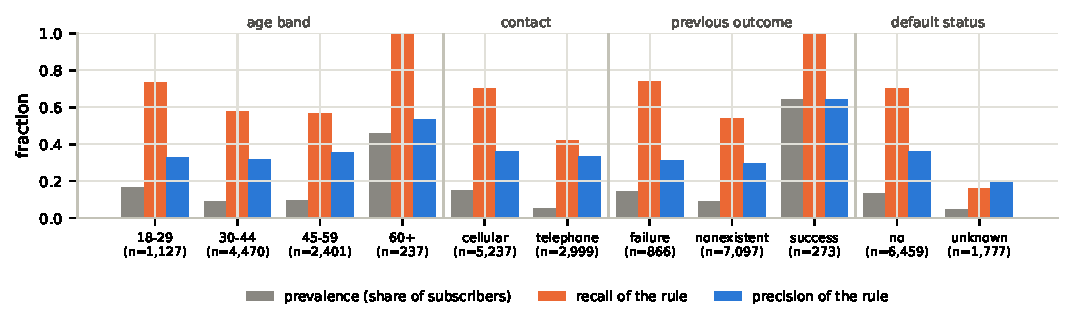
\includegraphics[width=0.95\textwidth]{fig_subgroups.pdf}
\caption{Prevalence, recall and precision of the recommended rule (calibrated GB, $t^\star=0.10$) by age band, contact channel, previous outcome and default status on the test set.}
\label{fig:sub}
\end{figure*}

\begin{table*}[!t]
\caption{Performance of the recommended rule (calibrated GB, $t^\star=0.10$) by subgroup on the test set. AP is omitted for groups with fewer than 20 subscribers.}
\label{tab:subgroups}
\centering\scriptsize
\begin{tabular}{lrrrrrrrr}
\toprule
variable & level & n & prevalence & call rate & recall & precision & AP & mean p\_hat \\
\midrule
age band & 18-29 & 1127 & 0.163 & 0.364 & 0.734 & 0.329 & 0.435 & 0.162 \\
age band & 30-44 & 4470 & 0.091 & 0.165 & 0.578 & 0.320 & 0.413 & 0.095 \\
age band & 45-59 & 2401 & 0.095 & 0.150 & 0.566 & 0.357 & 0.478 & 0.092 \\
age band & 60+ & 237 & 0.456 & 0.844 & 0.991 & 0.535 & 0.754 & 0.408 \\
contact & cellular & 5237 & 0.147 & 0.288 & 0.702 & 0.358 & 0.503 & 0.145 \\
contact & telephone & 2999 & 0.053 & 0.067 & 0.421 & 0.332 & 0.336 & 0.055 \\
previous outcome & failure & 866 & 0.145 & 0.342 & 0.738 & 0.314 & 0.389 & 0.150 \\
previous outcome & nonexistent & 7097 & 0.088 & 0.161 & 0.541 & 0.297 & 0.350 & 0.087 \\
previous outcome & success & 273 & 0.641 & 1.000 & 1.000 & 0.641 & 0.800 & 0.656 \\
education & basic.4y & 839 & 0.100 & 0.136 & 0.679 & 0.500 & 0.617 & 0.094 \\
education & basic.6y & 431 & 0.093 & 0.095 & 0.450 & 0.439 & 0.491 & 0.081 \\
education & basic.9y & 1186 & 0.082 & 0.122 & 0.433 & 0.290 & 0.300 & 0.077 \\
education & high.school & 1938 & 0.110 & 0.200 & 0.601 & 0.331 & 0.431 & 0.106 \\
education & illiterate & 1 & 0.000 & 0.000 & -- & -- & -- & 0.029 \\
education & professional.course & 1033 & 0.108 & 0.221 & 0.705 & 0.346 & 0.516 & 0.115 \\
education & university.degree & 2478 & 0.130 & 0.280 & 0.731 & 0.340 & 0.482 & 0.139 \\
education & unknown & 330 & 0.179 & 0.303 & 0.797 & 0.470 & 0.637 & 0.158 \\
job & admin. & 2156 & 0.131 & 0.271 & 0.749 & 0.363 & 0.517 & 0.134 \\
job & blue-collar & 1809 & 0.077 & 0.082 & 0.379 & 0.356 & 0.309 & 0.066 \\
job & entrepreneur & 254 & 0.091 & 0.114 & 0.348 & 0.276 & 0.333 & 0.078 \\
job & housemaid & 197 & 0.102 & 0.147 & 0.650 & 0.448 & 0.644 & 0.098 \\
job & management & 578 & 0.121 & 0.225 & 0.686 & 0.369 & 0.504 & 0.114 \\
job & retired & 353 & 0.280 & 0.535 & 0.889 & 0.466 & 0.742 & 0.261 \\
job & self-employed & 291 & 0.086 & 0.206 & 0.640 & 0.267 & 0.334 & 0.096 \\
job & services & 798 & 0.070 & 0.099 & 0.321 & 0.228 & 0.335 & 0.075 \\
job & student & 183 & 0.290 & 0.721 & 0.925 & 0.371 & 0.634 & 0.291 \\
job & technician & 1341 & 0.092 & 0.195 & 0.597 & 0.284 & 0.344 & 0.107 \\
job & unemployed & 211 & 0.152 & 0.265 & 0.812 & 0.464 & 0.655 & 0.149 \\
job & unknown & 65 & 0.046 & 0.185 & 0.667 & 0.167 & -- & 0.092 \\
default status & no & 6459 & 0.131 & 0.255 & 0.702 & 0.361 & 0.503 & 0.129 \\
default status & unknown & 1777 & 0.046 & 0.037 & 0.159 & 0.197 & 0.167 & 0.052 \\
\bottomrule
\end{tabular}
\end{table*}

\end{document}
